% !TEX root =../ECE343_Slides_Rogers.tex


%%%%%%%%%%%%%%%%%%%%%%%%%%%%%%%%%%%%%%%%%%%%%%%%%%%%%%
%%%%%%%%%%%%%%%%%%%%%%%%%%%%%%%%%%%%%%%%%%%%%%%%%%%%%%

\section{Schedule}
%\renewcommand{\arraystretch}{1}
%\begin{frame}{}
%	\begin{textblock}{14}(0.5,1.75)
%	\def\myfontsize{footnotesize}
%	
\setcounter{mylnum}{1}
\begin{center}
\begin{\myfontsize}
\begin{tabular}{| c | l | c | l |}
\hline
\textbf{Lesson} 		  	& \textbf{Topics}             & \pbox{5cm}{\textbf{Reading}}	& \textbf{Notes}		\\ \hline\hline
\ifnum\lessonNum=\value{mylnum} \rowcolor{green!20!white}\fi
	\themylnum  
	& Course Overview  \& Introduction		
	& Ch.1 
	&  LO 1.1-1.2 
	\stepcounter{mylnum}\\ \hline \hline
\rowcolor{gray!20!white}\multicolumn{4}{| c |}{\textbf{Chapter 2: Electric and Magnetic Fields}}	\\ \hline\hline
\ifnum\lessonNum=\value{mylnum} \rowcolor{green!20!white}\fi
	\themylnum 	
	& Fields, Parameters, Field Quantities	
	& Ch. 2	
	& LO 2.1-2.2			
\stepcounter{mylnum}\\ \hline\hline
\rowcolor{gray!20!white}\multicolumn{4}{| c |}{\textbf{Chapter 3: Transmission Lines}}	 \\ \hline\hline	
\ifnum\lessonNum=\value{mylnum} \rowcolor{green!20!white}\fi
	\themylnum 	
	& Lumped Element Model				
	& 3.1-3.4 
	& LO 3.1		
\stepcounter{mylnum}\\ \hline
\ifnum\lessonNum=\value{mylnum} \rowcolor{green!20!white}\fi
	\themylnum 	
	& Telegrapher's Equations
	& 3.5-3.6
	&  LO 3.1	
\stepcounter{mylnum}\\ \hline
\ifnum\lessonNum=\value{mylnum} \rowcolor{green!20!white}\fi
	\themylnum 	
	&  Characteristic Impedance \& Wave Propagation	
	& 3.7-3.9		
	& LO 3.2						
\stepcounter{mylnum}\\ \hline
\ifnum\lessonNum=\value{mylnum} \rowcolor{green!20!white}\fi
	\themylnum 	
	& Coaxial,  Reflection Coefficient, VSWR	
	& 3.10,3.12-3.14	
	& LO 3.2-3.3		
\stepcounter{mylnum}\\ \hline 
\ifnum\lessonNum=\value{mylnum} \rowcolor{green!20!white}\fi
	\themylnum 	
	&  Terminated Transmission Lines	
	&  3.15,3.17-3.19
	& LO 3.4		
\stepcounter{mylnum}\\ \hline 
\ifnum\lessonNum=\value{mylnum} \rowcolor{green!20!white}\fi
	\themylnum	
	& Impedance Matching	
	& 3.21-3.23
	& LO 3.4 			
\stepcounter{mylnum}\\ \hline 
\ifnum\lessonNum=\value{mylnum} \rowcolor{green!20!white}\fi
	\themylnum  
	& Impedance Matching	
	& 3.21-3.23
	& LO 3.4		
\stepcounter{mylnum}\\ \hline 
\ifnum\lessonNum=\value{mylnum} \rowcolor{green!20!white}\fi
	\themylnum	
	& Smith Charts
	& Supplemental
	& LO 3.5
\stepcounter{mylnum}\\ \hline 
\ifnum\lessonNum=\value{mylnum} \rowcolor{green!20!white}\fi
	\themylnum	
	& Smith Charts
	& Supplemental 
	& LO 3.5					
\stepcounter{mylnum}\\ \hline 
\ifnum\lessonNum=\value{mylnum} \rowcolor{green!20!white}\fi
	\themylnum	
	& Smith Charts
	& Supplemental 
	& LO 3.5	
\stepcounter{mylnum}\\ \hline 
\ifnum\lessonNum=\value{mylnum} \rowcolor{green!20!white}\fi
	\themylnum	
	& Smith Charts
	& Supplemental 
	& LO 3.5	
\stepcounter{mylnum}\\ \hline 

\ifnum\lessonNum=\value{mylnum} \rowcolor{green!20!white}\fi
	\themylnum	
	& Transients		
	& Supplemental 
	& LO 3.6	 
\stepcounter{mylnum}\\ \hline \hline
\ifnum\lessonNum=\value{mylnum} \rowcolor{green!20!white}\fi
	\themylnum 	
	& Flex Day
	& 
	& 	
\stepcounter{mylnum}\\ \hline 
\ifnum\lessonNum=\value{mylnum} \rowcolor{green!20!white}\fi
	\themylnum 	
	& Reflection/Transmission Coefficient Lab
	& Lab Packet
	& LO 3.7		
\stepcounter{mylnum}\\ \hline 
\ifnum\lessonNum=\value{mylnum} \rowcolor{green!20!white}\fi
	\themylnum 	
	& Reflection/Transmission Coefficient Lab
	& Lab Packet
	& LO 3.7		
\stepcounter{mylnum}\\ \hline 
\rowcolor{gray!20!white}\multicolumn{4}{| c |}{\textbf{Chapter 4: Vector Analysis}} \\ \hline\hline
\ifnum\lessonNum=\value{mylnum} \rowcolor{green!20!white}\fi
	\themylnum	
	& Vector \& Coordinate System Review
	& Ch. 4
	&LO 4.1-4.4 \textbf{GR 1 due}	
\stepcounter{mylnum}\\ \hline 
\rowcolor{gray!20!white}\multicolumn{4}{| c |}{\textbf{Chapter 5: Electrostatics}}\\ \hline\hline
\ifnum\lessonNum=\value{mylnum} \rowcolor{green!20!white}\fi
	\themylnum	
	& Coulomb's Law
	& 5.1-5.3
	& LO 5.1
\stepcounter{mylnum}\\ \hline 
\ifnum\lessonNum=\value{mylnum} \rowcolor{green!20!white}\fi
	\themylnum	
	& Surface and Volume Charge			
	& 5.4
	& LO 5.1
\stepcounter{mylnum}\\ \hline 
\ifnum\lessonNum=\value{mylnum} \rowcolor{green!20!white}\fi
	\themylnum	
	& Gauss' Law (Integral Form)
	& 5.5-5.6
	& LO 5.2		 					
\stepcounter{mylnum}\\ \hline 
\ifnum\lessonNum=\value{mylnum} \rowcolor{green!20!white}\fi
	\themylnum	
	& Gauss' Law (Differential Form)		
	& 5.7-5.8
	& LO 5.2	 	
\stepcounter{mylnum}\\ \hline 
\ifnum\lessonNum=\value{mylnum} \rowcolor{green!20!white}\fi
	\themylnum	
	& Electric Potential	
	& 5.9-5.10, 5.15
	&  LO 5.3	
\stepcounter{mylnum}\\ \hline 
% <---- line 129 should be 20 lessons, based on 6 lines per lesson, starting at line 9 
\end{tabular}			
\end{\myfontsize}
\end{center}

%	\end{textblock}
%\end{frame}


%%%%%%%%%%%%%%%%%%%%%%%%%%%%%%%%%%%%%%%%%%%%%%%%%%%%%%%%%%%%%%%%%%
%%%%%%%%%%%%%%%%%%%%%%%%%%%%%%%%%%%%%%%%%%%%%%%%%%%%%%%%%%%%%%%%%%

\begin{frame}{}
\renewcommand{\arraystretch}{1}
	\begin{textblock}{14}(0.5,1.75)
	\def\myfontsize{footnotesize}
	\setcounter{mylnum}{24}
%\def\myfontsize{normalsize}
\begin{center}
\begin{\myfontsize}
\begin{tabular}{| c | l | c | l |}
\hline
\textbf{Lesson} 		  	& \textbf{Topics}             & \pbox{5cm}{\textbf{Reading}}	& \textbf{Notes}		\\ \hline\hline
\ifnum\lessonNum=\value{mylnum} \rowcolor{green!20!white}\fi
	\themylnum  
	& BVP (Capacitor, Coax), Electric Potential	
	& 5.16
	&  LO 5.3  
\stepcounter{mylnum}\\ \hline \hline
\ifnum\lessonNum=\value{mylnum} \rowcolor{green!20!white}\fi
	\themylnum 	
	& Electric Boundary Conditions
	& 5.18-5.22	
	& LO 5.4			
\stepcounter{mylnum}\\ \hline
\ifnum\lessonNum=\value{mylnum} \rowcolor{green!20!white}\fi
	\themylnum 	
	& BC's/Capacitance			
	& 5.23-5.24
	& 	
\stepcounter{mylnum}\\ \hline
\ifnum\lessonNum=\value{mylnum} \rowcolor{green!20!white}\fi
	\themylnum 	
	& Electrostatic Lab			
	& Lab packet
	& 	
\stepcounter{mylnum}\\ \hline
\rowcolor{gray!20!white}\multicolumn{4}{| c |}{\textbf{Chapter 6: Steady Current \& Conductivity}}	\\ \hline\hline
\ifnum\lessonNum=\value{mylnum} \rowcolor{green!20!white}\fi
	\themylnum 	
	& Current density, Conductivity, Resistance
	& Ch. 6
	&   					
\stepcounter{mylnum}\\ \hline\hline
\rowcolor{gray!20!white}\multicolumn{4}{| c |}{\textbf{Chapter 7: Magnetostatics}}						\\ \hline\hline
\ifnum\lessonNum=\value{mylnum} \rowcolor{green!20!white}\fi
	\themylnum 	
	&  Magnetic Fields, Gauss' Law for Magnetism	
	& 7.1-7.3		
	&LO 7.1-7.2 \textbf{GR 2} 				
\stepcounter{mylnum}\\ \hline
\ifnum\lessonNum=\value{mylnum} \rowcolor{green!20!white}\fi
	\themylnum 	
	& Ampere's Law 	
	& 7.4-7.5, 7.9
	& LO 7.3		
\stepcounter{mylnum}\\ \hline 
\ifnum\lessonNum=\value{mylnum} \rowcolor{green!20!white}\fi
	\themylnum 	
	&  Ampere's Law Applied
	&  7.6-7.8
	& LO 7.3
\stepcounter{mylnum}\\ \hline 
\ifnum\lessonNum=\value{mylnum} \rowcolor{green!20!white}\fi
	\themylnum	
	& Magnetic Boundary Conditions	
	& 7.10-7.14	
	& LO 7.4 		
\stepcounter{mylnum}\\ \hline 
\ifnum\lessonNum=\value{mylnum} \rowcolor{green!20!white}\fi
	\themylnum  
	& Magnetostatics Lab
	& Lab packet
	&  		
\stepcounter{mylnum}\\ \hline \hline
\rowcolor{gray!20!white}\multicolumn{4}{| c |}{\textbf{Chapter 8: Time-Varying Fields}}					\\ \hline\hline
\ifnum\lessonNum=\value{mylnum} \rowcolor{green!20!white}\fi
	\themylnum 	
	& Faraday's Law, Displacement Current, Maxwell Eqns
	& 8.3, 8.8, 8.9
	& LO 8.1
\stepcounter{mylnum}\\ \hline 
\ifnum\lessonNum=\value{mylnum} \rowcolor{green!20!white}\fi
	\themylnum	
	& Faraday's Law, Displacement Current, Maxwell Eqns 
	&  8.3, 8.8, 8.9
	& LO 8.2-8.3
\stepcounter{mylnum}\\ \hline 

\rowcolor{gray!20!white}\multicolumn{4}{| c |}{\textbf{Chapter 9: Plane Waves in Lossless Media}}					\\ \hline\hline
\ifnum\lessonNum=\value{mylnum} \rowcolor{green!20!white}\fi
	\themylnum	
	& Maxwell's Equations in lossless, source-free region		
	& 9.1-9.2
	& LO 9.1	 
\stepcounter{mylnum}\\ \hline
\ifnum\lessonNum=\value{mylnum} \rowcolor{green!20!white}\fi
	\themylnum	
	& Maxwell's Equations in lossless, source-free region		
	& 9.1-9.2
	& LO 9.1	 
\stepcounter{mylnum}\\ \hline
%\ifnum\lessonNum=\value{mylnum} \rowcolor{green!20!white}\fi
%	\themylnum	
%	& Flex day
%	& 
%	& \textbf{GR 3}			 					
%\stepcounter{mylnum}\\ \hline 
\ifnum\lessonNum=\value{mylnum} \rowcolor{green!20!white}\fi
	\themylnum	
	& Uniform Plane Waves \& Polarization
	& 9.4-9.6
	& LO 9.2-9.3			
\stepcounter{mylnum}\\ \hline 
\ifnum\lessonNum=\value{mylnum} \rowcolor{green!20!white}\fi
	\themylnum	
	& Normal Incidence
	& Vol 2, 5.6-5.7
	&  LO 9.4-9.5
\stepcounter{mylnum}\\ \hline 
\ifnum\lessonNum=\value{mylnum} \rowcolor{green!20!white}\fi
	\themylnum	
	& Oblique Incidence			
	& Vol 2, 5.6-5.7
	& LO 9.5
\stepcounter{mylnum}\\ \hline 
\ifnum\lessonNum=\value{mylnum} \rowcolor{green!20!white}\fi
	\themylnum	
	& Oblique Incidence			
	& Vol 2, 5.6-5.7
	& LO 9.5
\stepcounter{mylnum}\\ \hline 
\ifnum\lessonNum=\value{mylnum} \rowcolor{green!20!white}\fi
	\themylnum	
	& Incidence Lab			
	& TBD
	& LO 9.5
\stepcounter{mylnum}\\ \hline 
%\ifnum\lessonNum=\value{mylnum} \rowcolor{green!20!white}\fi
%	\themylnum	
%	& Wrapup
%	& 
%	& 		 					
%\stepcounter{mylnum}\\ \hline 

\end{tabular}			
\end{\myfontsize}
\end{center}

	\end{textblock}
\end{frame}

%%%%%%%%%%%%%%%%%%%%%%%%%%%%%%%%%%%%%%%%%%%%%%%%%%%%%
%%%%%%%%%%%%%%%%%%%%%%%%%%%%%%%%%%%%%%%%%%%%%%%%%%%%%

\def\obja{ I can apply Coloumb's Law to use direct integration to calculate the electric field due to charge density in varoius geometries, including rectangular, cylindrical, and spherical coordinate systems. }
\def\objb{ I can apply the integral and differential forms of Gauss' Law to calculate the electric field due to charge density in various geometries, including rectangular, cylindrical, and spherical coordinate systems. }
\def\objc{ I can calculate the electric field from the scalar electric potential in a variety of geometries.}
\def\objd{ I can apply the electric field boundary conditions to calculate electric fields on both sides of a material boundary. }
\begin{frame}{Ch 5 Learning Objectives}
	\begin{textblock}{14}(0.5,2.5)
	\begin{myblock}[0.95]{}
	\begin{small}
	\begin{enumerate}[{5}.1]
		\ifnum\objNum=1
			\item \alert{ \obja }
		\else 
			\item \obja
		\fi 
		\ifnum\objNum=2
			\item \alert{ \objb }
		\else 
			\item \objb
		\fi 
		\ifnum\objNum=3
			\item \alert{ \objc }
		\else 
			\item \objc
		\fi 
		\ifnum\objNum=4
			\item \alert{ \objd }
		\else 
			\item \objd
		\fi 	
	\end{enumerate}
	\end{small}
	\end{myblock}
	\end{textblock}
\end{frame}

%%%%%%%%%%%%%%%%%%%%%%%%%%%%%%%%%%%%%%%%%%%%%%%%%%%%%
%%%%%%%%%%%%%%%%%%%%%%%%%%%%%%%%%%%%%%%%%%%%%%%%%%%%%

% Gauss' Law

\begin{frame}{Gauss' Law}
\begin{textblock}{14.5}(0.5,2.5)

\begin{myblock}[0.9]{Definition}

The flux of the electric charge through a \textbf{closed} surface is equal to the enclosed charge.

\end{myblock}

\vspace{-12pt}

\begin{myblock}[0.9]{Integral \& Differential (Point) Forms}
\vspace{-12pt}
\eq{
	\oiint_S \vec{D} \mycdot \vec{dS}  = Q_{\text{enclosed}} \qquad
	\nabla\mycdot \vec{D} = \rho_V 
}
\vspace{-12pt}
\end{myblock}


\end{textblock}
\end{frame}

%%%%%%%%%%%%%%%%%%%%%%%%%%%%%%%%%%%%%%%%%%%%%%%%%%%%%%
%%%%%%%%%%%%%%%%%%%%%%%%%%%%%%%%%%%%%%%%%%%%%%%%%%%%%%
%%%%%%%%%%%%%%%%%%%%%%%%%%%%%%%%%%%%%%%%%%%%%%%%%%%%%%
%%%%%%%%%%%%%%%%%%%%%%%%%%%%%%%%%%%%%%%%%%%%%%%%%%%%%%
\begin{frame}{Gauss' Law: General Method}
\begin{textblock}{7}(0.5,3)

\tdplotsetmaincoords{60}{110}
\begin{tikzpicture}[scale=3,tdplot_main_coords]
	\coordinate (O) at (0,0,0);
	\coordinate (A) at (0, 0.63, 0.63);
	
    % spherical background
    \tdplotsetrotatedcoords{20}{80}{0}
    \draw [ball color=white,very thin,tdplot_rotated_coords] (0,0,0) circle (0.75) ;
    \draw[fill=black] (0,0,0) circle (1pt) node[above] {$Q$}; 
    
    % equator
    \draw [dashed] (0,0,0) circle (0.75) ;
	\draw[thick,-stealth] (0,0,0) -- (1.75,0,0) node[anchor=north east]{$x$};
	\draw[thick,-stealth] (0,0,0) -- (0,1.25,0) node[anchor=north west]{$y$};
	\draw[thick,-stealth] (0,0,0) -- (0,0,1.25) node[anchor=south]{$z$};
	
	\draw[thick, red, -stealth] (O) -- (A) node[right, red] {$a$};

\end{tikzpicture}
\end{textblock}
\begin{textblock}{7}(8.5,2)

\begin{myblock}[0.95]{Method}
	\begin{enumerate}
	\setlength\itemsep{12pt}
		\item Draw Gaussian Surface ($\vec{dS}$)
		
		\item Determine symmetry
		
		\item Solve Left Integral:
		
		\vspace{-12pt}

		\eq{
			\oiint_S \varepsilon\vec{E} \mycdot \vec{dS}
		}
		
		\item Determine charge enclosed, $Q_{\text{encl}}$
		
%		\item Solve for $\vec{E}$
				
	\end{enumerate}
\end{myblock}
	
\end{textblock}
\end{frame}

%%%%%%%%%%%%%%%%%%%%%%%%%%%%%%%%%%%%%%%%%%%%%%%%%%%%%%
%%%%%%%%%%%%%%%%%%%%%%%%%%%%%%%%%%%%%%%%%%%%%%%%%%%%%%
%%%%%%%%%%%%%%%%%%%%%%%%%%%%%%%%%%%%%%%%%%%%%%%%%%%%%%
%%%%%%%%%%%%%%%%%%%%%%%%%%%%%%%%%%%%%%%%%%%%%%%%%%%%%%
\begin{frame}{Gauss' Law: Point Charge}

\begin{textblock}{7}(0.5,3)
\scalebox{0.75}{
\tdplotsetmaincoords{60}{110}
\begin{tikzpicture}[scale=3,tdplot_main_coords]
	\coordinate (O) at (0,0,0);
	\coordinate (A) at (0, 0.63, 0.63);
	
    % spherical background
    \tdplotsetrotatedcoords{20}{80}{0}
    \draw [ball color=white,very thin,tdplot_rotated_coords] (0,0,0) circle (0.75) ;
    \draw[fill=red!30!white, red] (0,0,0) circle (1pt) node[above] {$Q$}; 
    
    % equator
    \draw [dashed] (0,0,0) circle (0.75) ;
	\draw[thick,-stealth] (0,0,0) -- (1.75,0,0) node[anchor=north east]{$x$};
	\draw[thick,-stealth] (0,0,0) -- (0,1.25,0) node[anchor=north west]{$y$};
	\draw[thick,-stealth] (0,0,0) -- (0,0,1.25) node[anchor=south]{$z$};
	
	\draw[thick, black,dashed] (O) -- (A) node[midway, below, black] {$a$};

\end{tikzpicture}
} % end scalebox
\end{textblock}

\begin{textblock}{7}(7.5,3)
%
%\begin{myblock}[0.95]{Find $\vec{E}$ Everywhere}
%	\vspace{-12pt}
	
	\visible<0|handout:1>{
	\alert{
	\eq{
			\oiint_S \vec{D} &= Q_{\text{enclosed}} \\
			\implies \vec{dS} &= \hat{r} r^2\sinp{\theta}d\theta d\phi \\
			\implies \vec{D} &= \varepsilon\vec{E} = \varepsilon\lb \rhat E_r + \thetahat E_{\theta} + \phihat E_{\phi} \rb \\
			\vec{D} \mycdot \vec{dS} &= \varepsilon E_r r^2\sinp{\theta}d\theta d\phi \\
			\oiint_S \vec{D} \mycdot \vec{dS} 
			&= \varepsilon E_r r^2 \int_0^{2\pi} \int_0^\pi \sinp{\theta} d\theta d\phi \\
			&= \varepsilon E_r r^2 (2)(2\pi) \\
			&= 4\pi\varepsilon E_r r^2
	} % end eq
	} %end alert
	} % end visible
%	\vspace{2in}
%
%\end{myblock}
	
\end{textblock}
\end{frame}


%%%%%%%%%%%%%%%%%%%%%%%%%%%%%%%%%%%%%%%%%%%%%%%%%%%%%%
%%%%%%%%%%%%%%%%%%%%%%%%%%%%%%%%%%%%%%%%%%%%%%%%%%%%%%


\begin{frame}{Gauss' Law: Line Charge}
\begin{textblock}{7}(0.5,4)
\begin{tikzpicture}[scale=0.7]
		\def\qonex{0}
		\def\qoney{3}
		\def\qtwox{0}
		\def\qtwoy{-2}
		\def\qthreex{4}
		\def\qthreey{0}
		\begin{axis}[ 
		domain=-5:5,
%		samples=200, 
%		xmin=-1, 
		xmax=2.5, 
		ymax=3.5,
		ymin=-3.5,
%		title={Single Square Pulse, $\Pi (\frac{t}{\tau})$},
%		scaled x ticks=base 10:6,
%		xtick scale label code/.code={},
%		minor x tick num = 5,
%		minor y tick num = 5,
		ytick={-3,3},
		yticklabels={-a,a},
		xtick=\empty,
%		xticklabels={$\rho$},
		xlabel={$\rho$},
		ylabel={$z$},
		axis y line = middle,
		axis x line = middle,
		x label style={xshift=0.5cm},
		x label style={yshift=-0.25cm},
		y label style ={xshift=-0.75cm},
		y label style = {yshift =0.5cm},
		yticklabel shift=0.5cm,
		clip=false,
		]
		\node[cylinder, shape border rotate=90, draw, minimum height=6.5cm, minimum width=0.5cm] at (0,0) {};
		\addplot[ultra thick, red] coordinates {(0,-3)(0,3)};
		\node[red] at (-0.5,0) {$\rho_L$};
		
		\end{axis}
\end{tikzpicture}
\end{textblock}
\begin{textblock}{7}(8,2.25)

%\begin{myblock}[0.95]{Find $\vec{E}$ Everywhere}
%	\vspace{-12pt}
	\visible<0|handout:1>{
	\alert{
	\begin{small}
	\eq{
%			\oiint_S \vec{D} &= Q_{\text{enclosed}} \\
			&\oiint_S \vec{E}\mycdot\vec{dS}  = \dfrac{Q_{\text{enclosed}}}{\varepsilon} \\
			&\int_{\text{top}} \vec{E} \mycdot \vec{dS} 
			+\int_{\text{bottom}} \vec{E} \mycdot \vec{dS} \\
			&+\int_{\text{side}} \vec{E} \mycdot \vec{dS} = \dfrac{Q_{\text{enclosed}}}{\varepsilon} \\
			\implies &\vec{E} = \rhohat E_{\rho} + \phihat E_{\phi} + \zhat E_{z} \\
			\implies &\vec{dS}  = \rhohat \rho d\phi dz \\
			\implies &E_{\rho} \int_{-a}^{a} \int_0^{2\pi} \rho d\phi dz = \dfrac{Q_{\text{enclosed}}}{\varepsilon} \\
			&E_{\rho} (2a) (2\pi)\rho = \dfrac{Q_{\text{enclosed}}}{\varepsilon} \\
			\implies &\vec{E} = \rhohat E_{\rho} = \dfrac{Q_{enclosed}}{4a\pi \varepsilon\rho}
	} % end eq
	\end{small}
	} %end alert
	} % end visible
%	\vspace{1.5in}
	
%\end{myblock}
	
\end{textblock}
\end{frame}

%%%%%%%%%%%%%%%%%%%%%%%%%%%%%%%%%%%%%%%%%%%%%%%%%%%%%%
%%%%%%%%%%%%%%%%%%%%%%%%%%%%%%%%%%%%%%%%%%%%%%%%%%%%%%


\begin{frame}{Gauss' Law: Line Charge (cont'd)}
\begin{textblock}{7}(0.5,4)
\begin{tikzpicture}[scale=0.7]
		\def\qonex{0}
		\def\qoney{3}
		\def\qtwox{0}
		\def\qtwoy{-2}
		\def\qthreex{4}
		\def\qthreey{0}
		\begin{axis}[ 
		domain=-5:5,
%		samples=200, 
%		xmin=-1, 
		xmax=2.5, 
		ymax=3.5,
		ymin=-3.5,
%		title={Single Square Pulse, $\Pi (\frac{t}{\tau})$},
%		scaled x ticks=base 10:6,
%		xtick scale label code/.code={},
%		minor x tick num = 5,
%		minor y tick num = 5,
		ytick={-3,3},
		yticklabels={-a,a},
		xtick=\empty,
%		xticklabels={$\rho$},
		xlabel={$\rho$},
		ylabel={$z$},
		axis y line = middle,
		axis x line = middle,
		x label style={xshift=0.5cm},
		x label style={yshift=-0.25cm},
		y label style ={xshift=-0.75cm},
		y label style = {yshift =0.5cm},
		yticklabel shift=0.5cm,
		clip=false,
		]
		\node[cylinder, shape border rotate=90, draw, minimum height=6.5cm, minimum width=0.5cm] at (0,0) {};
		\addplot[ultra thick, red] coordinates {(0,-3)(0,3)};
		\node[red] at (-0.5,0) {$\rho_L$};
		
		\end{axis}
\end{tikzpicture}
\end{textblock}
\begin{textblock}{7}(8.25,3)

%\begin{myblock}[0.95]{Find $\vec{E}$ Everywhere}
%	\vspace{-12pt}
	\visible<0|handout:1>{
	\alert{
	\begin{small}
	\eq{
		 &\vec{E} = \dfrac{Q_{enclosed}}{4a\pi \varepsilon\rho} \\
		\implies &Q_{\text{enclosed}} = \int_{-a}^{a} \rho_L dz = 2a\rho_L \\
		\implies &\vec{E} = \dfrac{2a\rho_L}{4a\pi \varepsilon\rho} = \dfrac{\rho_L}{2\pi \varepsilon\rho} 
	} % end eq
	\end{small}
	} %end alert
	} % end visible
%	\vspace{1.5in}
	
%\end{myblock}
	
\end{textblock}
\end{frame}


% sheet charge
%%%%%%%%%%%%%%%%%%%%%%%%%%%%%%%%%%%%%%%%%%%%%%%%%%%%%%
%%%%%%%%%%%%%%%%%%%%%%%%%%%%%%%%%%%%%%%%%%%%%%%%%%%%%%

\begin{frame}{Gauss' Law: Sheet Charge}
\begin{textblock}{6.5}(0.5,3)
Find the Electric field everywhere from a sheet carrying a charge distribution of $\rho_S$. 
\scalebox{0.8}{
\tdplotsetmaincoords{70}{110}
	\begin{tikzpicture}[tdplot_main_coords]
	
	\draw[red, fill=red!30!white] (2,-2,0) -- (-2,-2,0) -- (-2,2,0) -- (2,2,0) -- cycle;
	\node[red] at (-1,-1,0) {$\rho_S (\text{\footnotesize{C/m}}^2)$};
	
	\pgfmathsetmacro{\cubex}{4}
	\pgfmathsetmacro{\cubey}{4}
	\pgfmathsetmacro{\cubez}{1}
	\draw[blue] (\cubex/2,\cubey/2,\cubez/2) -- ++(-\cubex,0,0) -- ++(0,-\cubey,0) -- ++(\cubex,0,0) -- cycle;
	\draw[blue] (\cubex/2,\cubey/2,\cubez/2) -- ++(0,0,-\cubez) -- ++(0,-\cubey,0) -- ++(0,0,\cubez) -- cycle;
	\draw[blue]  (\cubex/2,\cubey/2,\cubez/2)  -- ++(-\cubex,0,0) -- ++(0,0,-\cubez) -- ++(\cubex,0,0) -- cycle;
	
	\coordinate (O) at (0,0,0);
	\draw[thick, <->] (-3.5,0,0) -- (3.5,0,0) node[anchor=north east]{$x$};
	\draw[thick,<->] (0,-2.5,0) --(0,3,0) node[anchor=north west]{$y$}; 
	\draw[thick,->] (0,0,0) --(0,0,3) node[anchor=south]{$z$}; 

	\node[below right] at (2,0,0) {a};
	\node[below right] at (-2,0,0) {-a};
	\node[above right] at (0,2,0) {b};
	\node[above right] at (0,-2,0) {-b};

	\end{tikzpicture}
	} % end scalebox
\end{textblock}

\begin{textblock}{7}(7.5,2.5)

%\begin{myblock}[0.94]{Find $\vec{E}$ Everywhere}
%	\vspace{-12pt}
%	
	\visible<0|handout:1>{
	\alert{
	\begin{small}
	\eq{
			&\oiint_S \vec{E}\mycdot\vec{dS} = \dfrac{Q_{\text{enclosed}}}{\varepsilon} \\
			&\int_{\text{top}} \vec{E} \mycdot \vec{dS} 
			+\int_{\text{bottom}} \vec{E} \mycdot \vec{dS} \\
			&+\int_{\text{sides}} \vec{E} \mycdot \vec{dS} = \dfrac{Q_{\text{enclosed}}}{\varepsilon} \\
			&\text{Top}\longrightarrow\vec{dS} = \zhat dxdy \\
			&\implies \int_{-b}^{b}\int_{-a}^{a} \lp \xhat E_x + \yhat E_y + \zhat E_z \rp \mycdot \lp \zhat dxdy \rp\\
			&\text{Bottom}\longrightarrow\vec{dS} = -\zhat dxdy \\
			&\implies \int_{-b}^{b}\int_{-a}^{a} \lp \xhat E_x + \yhat E_y - \zhat E_z \rp \mycdot \lp -\zhat dxdy \rp \\
	} % end eq
	\end{small}
	} %end alert
	} % end visible
%
%\vspace{1.5in}
%\end{myblock}
	
\end{textblock}
\end{frame}

%%%%%%%%%%%%%%%%%%%%%%%%%%%%%%%%%%%%%%%%%%%%%%%%%%%%%%
%%%%%%%%%%%%%%%%%%%%%%%%%%%%%%%%%%%%%%%%%%%%%%%%%%%%%%

\begin{frame}{Gauss' Law: Sheet Charge (cont'd)}
\begin{textblock}{6.5}(0.5,3)
Find the Electric field everywhere from a sheet carrying a charge distribution of $\rho_S$. 
\scalebox{0.8}{
\tdplotsetmaincoords{70}{110}
	\begin{tikzpicture}[tdplot_main_coords]
	
	\draw[red, fill=red!30!white] (2,-2,0) -- (-2,-2,0) -- (-2,2,0) -- (2,2,0) -- cycle;
	\node[red] at (-1,-1,0) {$\rho_S (\text{\footnotesize{C/m}}^2)$};
	
	\pgfmathsetmacro{\cubex}{4}
	\pgfmathsetmacro{\cubey}{4}
	\pgfmathsetmacro{\cubez}{1}
	\draw[blue] (\cubex/2,\cubey/2,\cubez/2) -- ++(-\cubex,0,0) -- ++(0,-\cubey,0) -- ++(\cubex,0,0) -- cycle;
	\draw[blue] (\cubex/2,\cubey/2,\cubez/2) -- ++(0,0,-\cubez) -- ++(0,-\cubey,0) -- ++(0,0,\cubez) -- cycle;
	\draw[blue]  (\cubex/2,\cubey/2,\cubez/2)  -- ++(-\cubex,0,0) -- ++(0,0,-\cubez) -- ++(\cubex,0,0) -- cycle;
	
	\coordinate (O) at (0,0,0);
	\draw[thick, <->] (-3.5,0,0) -- (3.5,0,0) node[anchor=north east]{$x$};
	\draw[thick,<->] (0,-2.5,0) --(0,3,0) node[anchor=north west]{$y$}; 
	\draw[thick,->] (0,0,0) --(0,0,3) node[anchor=south]{$z$}; 

	\node[below right] at (2,0,0) {a};
	\node[below right] at (-2,0,0) {-a};
	\node[above right] at (0,2,0) {b};
	\node[above right] at (0,-2,0) {-b};

	\end{tikzpicture}
	} % end scalebox
\end{textblock}


\begin{textblock}{7}(8,2.5)

%\begin{myblock}[0.94]{Find $\vec{E}$ Everywhere}
%	\vspace{-12pt}
%	
	\visible<0|handout:1>{
	\alert{
	\begin{small}
	\eq{
			&\oiint_S \vec{E}\mycdot\vec{dS} = \dfrac{Q_{\text{enclosed}}}{\varepsilon} \\
			&\implies 2\int_{-b}^{b}\int_{-a}^{a} E_z dx dy = \dfrac{Q_{\text{enclosed}}}{\varepsilon}  \\
			&\implies (2E_z)(2a)(2b)   = \dfrac{Q_{\text{enclosed}}}{\varepsilon} \\
			&\implies 8E_z ab = \dfrac{(2a)(2b)\rho_S }{\varepsilon} \\
			&\vec{E} = \zhat E_z = \dfrac{\rho_S}{2\varepsilon}
	} % end eq
	\end{small}
	} %end alert
	} % end visible
%
%\vspace{1.5in}
%\end{myblock}
	
\end{textblock}
\end{frame}


% coaxial cable
%%%%%%%%%%%%%%%%%%%%%%%%%%%%%%%%%%%%%%%%%%%%%%%%%%%%%%
%%%%%%%%%%%%%%%%%%%%%%%%%%%%%%%%%%%%%%%%%%%%%%%%%%%%%%

\begin{frame}{Gauss' Law: Coaxial Cable}

\begin{textblock}{14.5}(0.5,3)
\scalebox{1.25}{
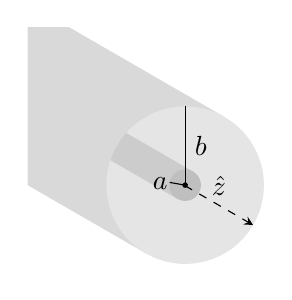
\begin{tikzpicture}[]
\clip (-2,-1.1) rectangle (1,2);
\begin{scope}[rotate=-30]
\fill[gray!30] (-3,-1) rectangle (0,1);
\fill[gray!20] (0,0) circle(1cm);
\begin{scope}
\clip(0,0) circle(1cm);
\fill[gray!40] (-3,-0.2) rectangle (0,0.2);
\fill[gray!50] (0,0) circle(2mm);
\fill[black] (0,0) circle (1pt); % origin
\end{scope}
\draw (120:0) -- node[right]{$b$}(120:1);
\draw (200:0) -- node[left]{$a$}(200:0.2);
\draw[-stealth, dashed] ([yshift=-0.5\pgflinewidth]0,0) -- node[above]{$\hat{z}$}([yshift=-0.5\pgflinewidth]1,0);
\end{scope}

\end{tikzpicture}%
} % end scalebox

\begin{tikzpicture}
\draw[pattern=north west lines, pattern color=gray!50!white] (0,0) circle (1.5);
\draw[black,fill=white] (0,0) circle (0.5);
\fill[black] (0,0) circle (1pt); % origin
\draw (120:0.5) -- node[right]{$b$}(120:1.5);
\draw (200:0) -- node[above]{$a$}(200:0.5);
\draw[dashed, -stealth] (90:0) -- (90:2);
 \draw[-stealth] (0,1.75) arc (90:120:1.5) node[above]{$\phi$};
\end{tikzpicture}
\end{textblock}

\begin{textblock}{7}(7,2.5)
	
	\visible<0|handout:1>{
	\alert{
	\begin{small}
	\eq{
			&\oiint_S \vec{E}\mycdot\vec{dS} = \dfrac{Q_{\text{enclosed}}}{\varepsilon} \\
			&\vec{E} = \rhohat E_{\rho} + \phihat E_{\phi} + \zhat E_z \\
			&\vec{dS} = \rhohat \rho dz d\phi \\
			&\implies \int_{0}^{2\pi} \int_{0}^{L} E_{\rho} \rho dz d\phi =  \dfrac{Q_{\text{enclosed}}}{\varepsilon} \\
			&\implies E_{\rho} \rho 2\pi L = \dfrac{1}{\varepsilon} \iiint \rho_V dV \\
			&\implies \rho_V = \dfrac{Q_{\text{tot}}}{\text{volume}} = \dfrac{Q_{\text{tot}}}{ \pi a^2 L} \\
			&\implies E_{\rho} \rho 2\pi L = \dfrac{1}{\varepsilon} \iiint \dfrac{Q_{\text{tot}}}{ \pi a^2 L} dV \\
			&\implies E_{\rho} \rho 2\pi L = \dfrac{Q_{\text{tot}}}{ \pi a^2 L \varepsilon} \int_{0}^{\rho_0} \rho d\rho \int_{0}^{2\pi} d\phi \int_{0}^{L} dz \\
	} % end eq
	\end{small}
	} %end alert
	} % end visible

	
\end{textblock}

\end{frame}

% coaxial cable
%%%%%%%%%%%%%%%%%%%%%%%%%%%%%%%%%%%%%%%%%%%%%%%%%%%%%%
%%%%%%%%%%%%%%%%%%%%%%%%%%%%%%%%%%%%%%%%%%%%%%%%%%%%%%

\begin{frame}{Gauss' Law: Coaxial Cable (cont'd)}

\begin{textblock}{14.5}(0.5,3)
\scalebox{1.25}{
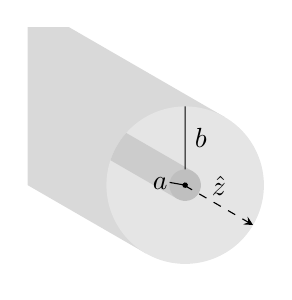
\begin{tikzpicture}[]
\clip (-2,-1.1) rectangle (1,2);
\begin{scope}[rotate=-30]
\fill[gray!30] (-3,-1) rectangle (0,1);
\fill[gray!20] (0,0) circle(1cm);
\begin{scope}
\clip(0,0) circle(1cm);
\fill[gray!40] (-3,-0.2) rectangle (0,0.2);
\fill[gray!50] (0,0) circle(2mm);
\fill[black] (0,0) circle (1pt); % origin
\end{scope}
\draw (120:0.2) -- node[right]{$b$}(120:1);
\draw (200:0) -- node[left]{$a$}(200:0.2);
\draw[-stealth, dashed] ([yshift=-0.5\pgflinewidth]0,0) -- node[above]{$\hat{z}$}([yshift=-0.5\pgflinewidth]1,0);
\end{scope}

\end{tikzpicture}%
} % end scalebox

\begin{tikzpicture}
\draw[pattern=north west lines, pattern color=gray!50!white] (0,0) circle (1.5);
\draw[black,fill=white] (0,0) circle (0.5);
\fill[black] (0,0) circle (1pt); % origin
\draw (120:0.5) -- node[right]{$b$}(120:1.5);
\draw (200:0) -- node[above]{$a$}(200:0.5);
\draw[dashed, -stealth] (90:0) -- (90:2);
 \draw[-stealth] (0,1.75) arc (90:120:1.5) node[above]{$\phi$};
\end{tikzpicture}
\end{textblock}

\begin{textblock}{7}(8,2.5)
	
	\visible<0|handout:1>{
	\alert{
	\begin{small}
	\eq{
			&\oiint_S \vec{E}\mycdot\vec{dS} = \dfrac{Q_{\text{enclosed}}}{\varepsilon} \\
			 &E_{\rho} \rho 2\pi L = \dfrac{Q_{\text{tot}}}{ \pi a^2 L \varepsilon} \lp \rho^2_0 \rp \lp 2\pi  \rp\lp L \rp \\
			 &E_{\rho} = \dfrac{Q_{\text{tot}} \rho^2_0}{2\pi\varepsilon a^2 L \rho} 
	} % end eq
	\end{small}
	} %end alert
	} % end visible

	
\end{textblock}

\end{frame}


% coaxial cable
%%%%%%%%%%%%%%%%%%%%%%%%%%%%%%%%%%%%%%%%%%%%%%%%%%%%%%
%%%%%%%%%%%%%%%%%%%%%%%%%%%%%%%%%%%%%%%%%%%%%%%%%%%%%%

\begin{frame}{Gauss' Law: Coaxial Cable (cont'd)}

\begin{textblock}{14.5}(0.5,3)
\scalebox{1.25}{
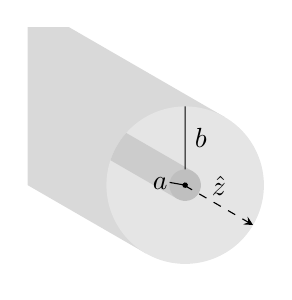
\begin{tikzpicture}[]
\clip (-2,-1.1) rectangle (1,2);
\begin{scope}[rotate=-30]
\fill[gray!30] (-3,-1) rectangle (0,1);
\fill[gray!20] (0,0) circle(1cm);
\begin{scope}
\clip(0,0) circle(1cm);
\fill[gray!40] (-3,-0.2) rectangle (0,0.2);
\fill[gray!50] (0,0) circle(2mm);
\fill[black] (0,0) circle (1pt); % origin
\end{scope}
\draw (120:0.2) -- node[right]{$b$}(120:1);
\draw (200:0) -- node[left]{$a$}(200:0.2);
\draw[-stealth, dashed] ([yshift=-0.5\pgflinewidth]0,0) -- node[above]{$\hat{z}$}([yshift=-0.5\pgflinewidth]1,0);
\end{scope}

\end{tikzpicture}%
} % end scalebox

\begin{tikzpicture}
\draw[pattern=north west lines, pattern color=gray!50!white] (0,0) circle (1.5);
\draw[black,fill=white] (0,0) circle (0.5);
\fill[black] (0,0) circle (1pt); % origin
\draw (120:0.5) -- node[right]{$b$}(120:1.5);
\draw (200:0) -- node[above]{$a$}(200:0.5);
\draw[dashed, -stealth] (90:0) -- (90:2);
 \draw[-stealth] (0,1.75) arc (90:120:1.5) node[above]{$\phi$};
\end{tikzpicture}
\end{textblock}

\begin{textblock}{7}(8,2.5)
	
%	\visible<0|handout:1>{
%	\alert{
%	\begin{small}
%	\eq{
%			&\text{Case 1: } 
%			 &E_{\rho} = \dfrac{Q_{\text{tot}} \rho^2_0}{2\pi\varepsilon a^2 L \rho} 
%	} % end eq
%	\end{small}
%	} %end alert
%	} % end visible

	
\end{textblock}

\end{frame}
%%%%%%%%%%%%%%%%%%%%%%%%%%%%%%%%%%%%%%%%%%%%%%%%%%%%%%
%%%%%%%%%%%%%%%%%%%%%%%%%%%%%%%%%%%%%%%%%%%%%%%%%%%%%%

\begin{frame}{Gauss' Law: Point (differential) Form}
\begin{textblock}{14.5}(0.5,3)

	\begin{myblock}[0.9]{Derivation}
		\eq{
			&\oiint \vec{D} \mycdot \vec{dS} = Q_{\text{encl}} \\
			&\iiint_V \nabla\mycdot \vec{D} dV = \iiint_V \rho_V dV  \\
			&\nabla \mycdot \vec{D} = \rho_V \\
			&\nabla \mycdot \vec{E} = \dfrac{\rho_V}{\varepsilon} \\
		}
	\vspace{-0.5in}

\end{myblock}

\end{textblock}
\end{frame}


%%%%%%%%%%%%%%%%%%%%%%%%%%%%%%%%%%%%%%%%%%%%%%%%%%%%%%
%%%%%%%%%%%%%%%%%%%%%%%%%%%%%%%%%%%%%%%%%%%%%%%%%%%%%%

\begin{frame}{Example}
\begin{textblock}{14.5}(0.5,3)
Given the following static electric field in free space, find the charge density ($\rho$) at the point $(2,-2,0)$

\vspace{-16pt}
\begin{small}
\eq{
	&\vec{E} (\vec{r} ) = \xhat A x^2 + \yhat B z + \zhat C x^2 z \longrightarrow  A = 3 \volts/\text{m}^3 \quad B = 2 \volts/\text{m}^3\quad C = 1 \volts/\text{m}^4
}
\end{small}

	\vspace{-24pt}
	\begin{myblock}[0.9]{Solution}
	\vspace{-18pt}
	\begin{small}
		\alert{
		\eq{
			\nabla\mycdot\vec{E} &= \dfrac{\rho}{\varepsilon_0} \\
			\varepsilon_0 \lb \partd{}{x} \lp 3x^2 \rp + \partd{}{y} \lp 2z \rp + \partd{}{z}\lp x^2 z \rp \rb &= \rho \\
			\varepsilon_0 \lp 6x + 0 + x^2 \rp &= \rho \\
			8.854\ee{-12}\text{F/m} \lb (6)(2) + 2^2 \rb &= \rho \\
			141.7 \text{pC/m}^3 = \rho
		}
		\vspace{-18pt}
		}
	\end{small}
	\end{myblock}

\end{textblock}
\end{frame}
\begin{comment}
\end{comment}